\chapter{Introduction}

\section{Background}
Our brain is characterized by a large number of cells that we rely on each and every second of every day to function properly. Neurons are one of the most important cells in the brain. Due to the complexity of the brain, brain
disorders can appear from very small cell to cell miscommunication. Brain cells are closely related, so miscommunication in one region can interrupt
other brain activity, which means that brain abnormalities can lead to systemic problems.
While there are many disorders that can affect the
brain, the most complex of these disorders are called Neurodegenerative Diseases(NDD).%[https://kids.frontiersin.org/article/10.3389/frym.2018.00070]
 As there is no proper cure for these diseases, so proper management of these diseases through Machine Learning and IoT can make the patient free enough by assistive living in-home health environment rather than staying in the hospital. Thus the caregiver can remotely monitor the patient through e-health environments and refer to a doctor in case of emergency.


\subsection{What is NDD}
Neurodegenerative Disease is a concept that leads to neurons death by blocking the nerve system which involves the brain and spinal cord and this is often incurable since neurons do not regenerate \cite{noor_detecting_2019}. The term neurodegenerative can be separated into neuro, meaning brain, and degenerative, meaning to break down, or to die. Neurodegenerative Disorders are the principal cause of the loss of interactions between healthy cells in the brain. In the human body, it can alter balance, movement (called ataxia), voice, breathing, memory (called dementia), intelligence and much more. \cite{bak_what_2012}. As the complexity of these neurodegenerative diseases are so much that the scientists could not find the cause of many of these diseases. The most commonly diagnosed neurodegenerative disorders include Parkinson's, Dementia, Alzheimer's, Huntington's, etc. Neurodegenerative diseases are considered often incurable to disease development without appropriate therapies, patients may also die. \cite{finkbeiner_huntingtons_2011}.







\subsection{Status of NDD in abroad}
A report made by World Health Organization (WHO) indicates that atleast 1 billion people throughout the world has been suffered from various neurological disorders such as neuro infections, headache, Parkinson, Alzheimer, Dementia, Schizophrenia, multiple sclerosis etc \cite{siuly_medical_2016}. The report also reveals that over 50 million people are suffering from Alzheimer's and other dementias, in the next 5 years which will be double \cite{noauthor_dementia_nodate}. After heart diseases, NDD is the second leading death factor with a minimum of 9 million deaths and 16.5\% of global deaths \cite{carroll_global_2019}. Nationality, sex are not the barrier of neurological disorders \cite{noauthor_who_nodate}. Even the suicide rate among these patients is five times higher than general people. Alzheimer’s Disease (AD) and Parkinson’s Disease (PD) are by far the most common form of NDDs and more than 5.4 million Americans were living with Alzheimer’s disease and it is predicted that an estimated 930,000 people in America will be living with Parkinson’s disease by 2020.

\subsection{Status of NDD in BD}
Researchers have found that NDD is responsible for 6\% of overall diseases and this level is high in developing and developed countries \cite{noauthor_journal_nodate}. The shortage of specialized equipment is a significant problem to be tackled in the treatment of neurological disorders. Since neurodegenerative diseases are very popular among all medical admissions at primary healthcare centers in Bangladesh and there is a shortage of facilities, numerous neurological issues are referred to the National Institute of Neurosciences and Hospital (NINS\&H) \cite{alam_neurological_2015}.


%\begin{equation*}
%    y=\int_x \sin(x)dx+\frac{a}{b}
%\end{equation*}

%where, $x$ x is input;

%\label{chap:GettingStarted}
\subsection{ML Approaches in Management of NDD}
%This section includes the overview of the report \cite{raytheon_2014,orend_2013,nps_tpo_2014}. 

Owing to the widespread popularity, Machine Learning (ML) techniques have been used for the biological data mining, image processing   \cite{ali2019segmentation}, decision support system \cite{kaiser2018tits}. 
Deep learning techniques are effective tools for the management of NDD that allow systems to learn from assessed data to build ways of making better and smarter choices that can improve patient management. This will help in processing medical data using multilayered neural networks, leading to increased prediction capabilities for many particular NDD management applications \cite{mahmud2018applications,mahmud2020dltools}. 
\subsection{IoT Approaches in Management of NDD}
On the other hand, the Internet of Things (IoT) is a network which contains physical objects such as sensors, software, and other technologies for communicating and sharing information over the web with other devices and applications. The number of Internet-connected
devices have exponential growth. A survey shows that in 2003, about 500 million computers have been wired to the internet, exceeding 12.5 billion in 2010. Researchers have predicted that there will be a minimum of 21 billion IoT devices by the year 2025. 
Internet of Things (IoT) devices introduce us with  modern wave of health care system with the idea of smart home appliances for elderly patients to monitor, manage, and motivate them \cite{lam_future_2010}. Numerous research projects have introduced a various number of smart system prototypes covering sensors, algorithms, and smart devices. 
Current IoT research focuses mainly on smart homes and connectivity systems that support remote control of electrical, heating and lighting appliances \cite{arunvivek_framework_2015}.
%

\section{Motivation}
Neurological disorders affect millions globally along with low and medium-income countries where there is a lack of facilities in the hospitals that’s why management of these diseases is important. This can reduce costs and extend the medical facilities by enhancing the quality of service. We want to develop a framework for patient monitoring and decision-making by using a home automation system so they can be managed in their own homes. Deep learning algorithm will be used to analyze the data we will get from the wearable device which will use the eHealth sensor, fall detection sensor, and GPS location.

%\begin{figure}
 %   \centering
  %  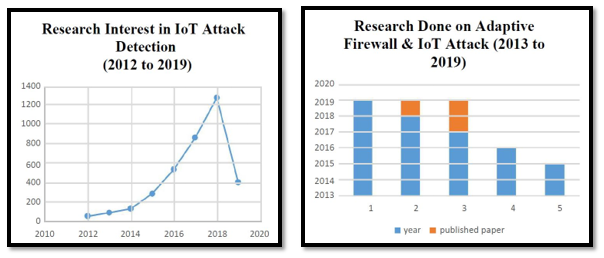
\includegraphics[scale=0.5]{Chap1/motivation.PNG}
   % \caption{Research Interest in Field of IoT}
    %\label{fig:motivation}
%\end{figure}

 %In figure \ref{fig:motivation} shows the existing research interest in IoT Attack Detection which is increasing day by day for last few years whereas for detecting attack concept of Adaptive Firewall is not so common and used term in this field. This drives us motivated to design adaptive firewall for attack detection and to block illegitimate traffic on IoT Network Model.


\section{Problem Statement}
Physicians/hospital experts/medical assistants need to collaborate with information technologies to use sophisticated tools to ensure a better level of clinical treatment as the computer-based patient management system progresses to support medical procedures and treatment at altitude. But there has not been much work in IoT based patient management. Analyzing the previous work results in this regard, the issues can be pointed out:\\
-	It is quite impossible to be with them always.\\
-	In the patient’s sudden illness there is no one to help her.\\
-	Can not measure the level of the patient's illness as always or sudden need.\\
-   Lack of optimum functioning, autonomy and self-care in interaction with broader physical, social and economic contexts.\\
-	Its quite costly exchanging information between doctors and patients.\\
-	Lack of consistency and coverage of medical services in the case of emergency.\\
-	The patient could not be monitored at home and the signals were sent to a hospital or the dearest person through the available communication line. 



\section{Objective}
Neurodegenerative disorders arise as nerve cells (neurons) in the brain and spinal cord appear to disintegrate. Modifications in these cells allow them to act abnormally and ultimately cause the cell to die. Most of these disorders are deadly. It is a big danger to people's health specially elderly people. Such age-dependent problems are becoming more common, partially because the elderly population has risen in recent years . So,  A modern and more effective \& strategic framework need to be developed to fight these destructive diseases. Our proposed system will serve the following objectives:


\begin{enumerate}[label=\roman*]
    

    \item To develop a system model to observe the NDD patient’s current state will result in the detection of any kind of fall.


    \item To support the accurate decision making using LSTM RNN. 

    \item To Compare three classifier and algorithms to find the appropriate ones for the fall event. 
    %\item Design a rule based and ANN based FIS to help SDN controller to evaluate specific attack probability and block the suspicious ones.
   % \item Maintaining the performance of the network.
\end{enumerate}

%This proposed model also answers the %following questions:\begin{enumerate}
%    \item What are the major challenges that have guided security in IoT?
 %   \item What is the best attack detection way for IoT network model?
  %  \item Is there any generalized approach for detecting different layer attack?
   % \item What is the best way to detect a single layer attack?
%\end{enumerate}

%\section{Assumptions \& Limitations}
%\begin{itemize}
   % \item No approach has been mentioned for network and application layer security.
%    \item No real time data has been used for the traffic analysis.
 %% \item No comparison among different IDS model has been analyzed so can’t be declared it as the optimal way. 
%    \item No performance measure of used Classifier is evaluated here.
%\end{itemize}
\section{Limitation}
The impediments of our project are written underneath: 
    \begin{enumerate}[label=\roman*]
        \item The cloud security of this project isn't created by us. The current security of the cloud is utilized here.
        \item We utilize various cameras that may not financially savvy.
        \item Sometimes impediments may make troubles identify an objective with the camera which can't identify the proper expressions.
    \end{enumerate}


%Analyzing the existing research works we have found that there are not much work in the field of management of NDD using ML and IoT. Thus we have found the following limitations in the existing researches.\\
%\begin{itemize}
    %\item  False alarm rate in emergency case is high as accuracy is low in  detection of Fall for the NDD patient.\\
    %\item
     %Most of the framework proposed by the researchers are only wearable device based or camera sensor based.\\
    %\item Privacy is the barrier in NDD management which is not mentioned in most of the work. 
%\end{itemize}

\section{Research Outline}
The remainder of the report is organized as follows: In Chapter II a writing study on related work is given including clarifications for the main terms utilized in this theory. Section III presents the framework model including framework design and flowchart of the working strategy of the whole framework model and also mentioned the required algorithm like Attention RNN. In Chapter IV system methodology is referenced. Numerical and Graphical Analysis of the system are referenced in Chapter V. Finally, In Chapter VI Conclusion and Future Work are referenced.


%\section{Research Outline}
%Rest of the report is structured as follows: In \textbf{Chapter \ref{chap:2}} a literature study on related work is given including explanations for the most important terms used in this thesis-basic concept and architecture of IoT Network Model. \textbf{Chapter III}  introduces system model including system architecture, algorithm and flowchart of working procedure of entire system model. \textbf{Chapter IV} explains the details of traffic analysis techniques, Feature Extraction and Selection mechanism and tools for this mechanism and reasoning how these mechanisms work for our model. \textbf{Chapter V} discusses about the simulation and model performance, to analysis result of the model it describes the basic mechanism of attack detection like Fuzzification, NSL KDD dataset, FIS, Defuzzification,Simulation and confusion matrix. Lastly in \textbf{Chapter VI} future work and conclusion is mentioned. 



\label{sec:EffSearch} 
\index{Search engines!using effectively} %index will be created
%The rest of this report is organized as follows.

